\documentclass[10pt,journal]{./IEEE_latex_class/IEEEtran}

% In order to reference go to http://truben.no/latex/bibtex/

% *** CITATION PACKAGES ***
\usepackage{cite}

% *** GRAPHICS RELATED PACKAGES ***
%
\ifCLASSINFOpdf
   \usepackage[pdftex]{graphicx}
  % declare the path(s) where your graphic files are
  \graphicspath{{./Figures/}}
  % and their extensions so you won't have to specify these with
  % every instance of \includegraphics
  \DeclareGraphicsExtensions{.pdf,.jpeg,.png}
\else
  % or other class option (dvipsone, dvipdf, if not using dvips). graphicx
  % will default to the driver specified in the system graphics.cfg if no
  % driver is specified.
  % \usepackage[dvips]{graphicx} 
  % declare the path(s) where your graphic files are 
  % \graphicspath{{../eps/}}   
  % and their extensions so you won't have to specify these with
  % every instance of \includegraphics
  % \DeclareGraphicsExtensions{.eps}
\fi


% *** MATH PACKAGES ***
\usepackage[cmex10]{amsmath}
\usepackage{amssymb}

% correct bad hyphenation here
\hyphenation{op-tical net-works semi-conduc-tor}

%  OTHER PACKAGES

\usepackage{float,amsfonts,multicol,fancyvrb,lastpage,ragged2e,url,color,lipsum,enumerate,todonotes,chemfig,fixltx2e}
\usepackage[caption=false]{subfig}



\begin{document}

%
% paper title
% can use linebreaks \\ within to get better formatting as desired
\title{Computational design of RNA-based oscillatory circuits}

\author{J.~Binysh
        \\ \IEEEmembership{* University of Warwick, Complexity Department}}

% The paper headers
\markboth{hi}%
{Computational design of RNA-based oscillatory circuits}

% make the title area
\maketitle

% This defines the title + page out of # of pages at the heading of the pages
\thispagestyle{empty}

\newcommand{\MYheader}{\smash{\scriptsize

\hfil\parbox[t][\height][t]{\textwidth}{\centering {\normalsize
Place conference title here}}\hfil\hbox{}}}
\makeatletter

\if@twoside
  \def\ps@headings{%
      \let\@oddfoot\@empty\let\@evenfoot\@empty
      \def\@evenhead{\small\thepage\hfil\leftmark\strut\vadjust{\vskip .1ex\hrule}}%
      \def\@oddhead{\small\rightmark\hfil\thepage\strut\vadjust{\vskip .1ex\hrule}}%
      \let\@mkboth\markboth
    \def\chaptermark##1{%
      \markboth{\scshape%
        \ifnum \c@secnumdepth >\m@ne
            \@chapapp\ \thechapter. \ %
        \fi
        ##1}{}}%
    \def\sectionmark##1{%
      \markright{\scshape%
        \ifnum \c@secnumdepth >\z@
          \thesection. \ %
        \fi
        ##1}}}
\else
  \def\ps@headings{%
    \let\@oddfoot\@empty
    \def\@oddhead{{\slshape\rightmark}\hfil\thepage\ of\ \pageref{LastPage} \strut\vadjust{\vskip .1ex\hrule}}%
    \let\@mkboth\markboth
    \def\chaptermark##1{%
      \markright{\scshape%
        \ifnum \c@secnumdepth >\m@ne
            \@chapapp\ \thechapter. \ %
        \fi
        ##1}}}
\fi
\makeatother

\makeatother

% make changes take effect
\pagestyle{headings}
% adjust as needed
%\addtolength{\footskip}{0\baselineskip}
%\addtolength{\textheight}{-0.1\baselineskip}

\begin{abstract}
genetic circuitry, RNA's offers an attractive alternative to more traditional methods, which typically involve using proteins to regulate DNA transcription. In comparison to proteins, it is relatively straightfor
\end{abstract}

\IEEEpeerreviewmaketitle


%%%
%%%
%%%
%%%
%%%
%NEW SECTION%
%%%
%%%
%%%
%%%


\section{Introduction}
\label{sec: Intro}
The process of gene expression can be briefly summarised as: DNA is read, and a copy of it is made, in the form of an RNA molecule (this is called \textit{transcription}). This RNA molecule (known as messenger RNA, or mRNA) makes its way to a piece of cellular machinery called the Ribosome, which reads it, and makes a protein - which protein is made depends on the DNA sequence originally read (\textit{translation}).  

 The path from genetic transcription to protein expression is naturally regulated in many ways \cite{MolecularBiology}. This regulation allows the cell to control protein expression, and so cell behaviour, in response to various environmental cues. The natural cell machinery which performs this regulation offers rich possibilities for modification, and an important goal within synthetic biology is to understand and manipulate it.

As well as acting as the intermediate between DNA and protein, RNA molecules play direct and important roles in regulating cell behaviour \cite{Isaacs2006}. For the synthetic biologist looking to engineer regulation of genetic circuitry, RNA's offers an attractive alternative to more traditional methods, which typically involve using proteins to regulate DNA transcription. In comparison to proteins, it is relatively straightforward to predict the structure and function of an RNA from its sequence using physiochemical models. Recently, this has been exploited to computationally design DNA sequences encoding synthetic sRNA's - small RNA's which do not code for a protein, but rather have some direct regulatory function -  with regulatory behaviour that can be predicted \cite{Rodrigo2013}\cite{Rodrigo2012}.

This report will focus on one such system, introduced in \cite{Rodrigo2012}. It will extend existing understanding of the system beyond the qualitative, by proposing a quantitative model of gene expression, in the form of a set of ODE's, and fitting it to available time series data to estimate the model's unknown parameters.

The report is structured as follows. In the remainder of this section we review the sRNA regulatory system we will consider. In section \ref{Results and Discussion} we propose a set of ODE's to model the system, and estimate its unknown parameters by fitting to time series data. Finally, in section \ref{Conclusions and Further work}, we conclude, and suggest directions for further work.


%NEW SUBSECTION%


\subsection{The sRNA regulatory system}
\label{The sRNA regulatory system}
In bacteria, one mechanism by which gene expression is regulated is as follows \cite{Soper2010}: In order for a bacterial mRNA to be translated into a protein, the Ribosome must initially bind to the mRNA (Fig. \ref{RBS}). This occurs at the Ribosome Binding Site (RBS) \cite{Shine1974}, a specific nucleotide sequence found on the mRNA. In an mRNA there is an untranslated region of nucleotides at the 5' end of the molecule (the UTR), upstream of the RBS. Translation may be self repressed by this `tail' of the mRNA folding over and binding across the RBS, forming a stem loop in the mRNA and preventing the Ribosome from binding (Fig. \ref{RBS}). This self repression may be released with an sRNA which binds to the same region on the mRNA - the new conformation of the sRNA:mRNA complex uncovers the RBS, allowing the Ribosome to bind. In summary, the presence of the sRNA positively regulates gene expresssion.

\begin{figure*}[t]
\centering
\includegraphics[trim = 30 600 30 0,page=4,clip = true]{pnas1203831109.pdf}
\caption{A logical AND gate formed from a self repressed mRNA, and an sRNA which uncovers its RBS. In this system, transcription of the sRNA (transRNA) and mRNA (5'-UTR,GFP) are controlled by two promoter regions, $P_{LtetO-1}$ and $P_{LlacO-1}$. These are disabled by the presence of two chemical repressors, TetR and LacI, found naturally in the strain of \textit{E. coli} discussed. These chemical repressors are themselves disabled by two chemicals, aTC and IPTG. In the notation of the diagram, a barred line indicates repression, and an arrowed line indicates production. We see a 'double negative' in aTc repressing TetR, which itself represses transcription of the sRNA (likewise for IPTG and the mRNA). Thus presence of the sRNA and mRNA are controlled by the presence of aTc and IPTG, which can be experimentally introduced to the cell.  Image reproduced from \cite{Rodrigo2012}.}
\label{ANDGate}
\end{figure*}

\begin{figure}[H]
\centering
\includegraphics[trim = 100 170 100 400,page=10,clip = true,scale = 0.6]{Appendix.pdf}
\caption{A mechanism by which sRNA's can regulate gene expression. Initially, the 5' UTR of the mRNA is folded over the RBS, forming a loop and blocking Ribosome binding. The sRNA binds to this mRNA, causing a conformational change which uncovers the RBS, and allows translation to occur.Image reproduced from \cite{Rodrigo2012} }
\label{RBS}
\end{figure}

\cite{Rodrigo2012} proposed a computational methodology to design general genetic circuits based on RNA interactions, and as a case study of the methodology chose to design a synthetic sRNA- mRNA pair capable of acting in the manner described above. The algorithm assumed an interaction scheme between the RNA's as shown in Fig. \ref{reactionscheme}. The two RNA's, originally in their own individually folded states, would initially interact via a small 'toehold' sequence of unpaired nucleotides to form an unstable transition state. This intermediate complex would then rapidly form a final, stable complex with the desired conformation. By suggesting sRNA and mRNA sequences which optimised this energy landscape, \cite{Rodrigo2012} suggested several devices which would form a stable hybrid with the RBS free, and experimentally validated their function in \textit{E. coli}, using an mRNA which codes for GFP for experimental ease (note the algorithm only optimises the 5' UTR of the mRNA, so the actual protein being coded for is unimportant).

\begin{figure}[H]
\centering
\includegraphics[trim = 60 630 300 30,page=2,clip = true]{pnas1203831109.pdf}
\caption{A network with an intuitively clear community structure, which is captured by the partition chosen, shown in gray. Image reproduced from \cite{Rodrigo2012}}
\label{reactionscheme}
\end{figure}


Further, by placing the concentrations of the sRNA and mRNA under the control of tuneable promoters, \cite{Rodrigo2012} constructs a logical AND gate from one of the proposed devices (RAJ11) \textit{in vivo} (Fig. \ref{ANDGate}). In this system, transcription of the designed sRNA and mRNA are placed under the control of promoter regions, $P_{LtetO-1}$ and $P_{LlacO-1}$ \cite{Lutz1997}. These are in turn controlled by two transcriptional repressors, TetR and LacI, which are naturally present in the strain of \text{E. coli} considered. These repressors disable the promoter regions, and so by default transcription of the RNA's is turned off, and no protein is produced. 
These repressors can themselves be disabled by the presence of two chemicals, aTC and IPTG, which can be introduced externally into the cell (Fig. \ref{ANDGate}).  So transcription of the two RNA's is indirectly controlled by the presence of two chemicals - if neither is present, sRNA and mRNA transcription is repressed, and no protein is produced. If only one is present, the AND gate remains off, either because there is no mRNA to be translated into protein, or because the mRNA is self repressed. But when both are present, the conformational change discussed above occurs, and protein is produced.
\todo[inline]{promoter?}

Although a qualitative understanding of this system exists \cite{Rodrigo2012}, it is of interest to attempt a quantitative understanding of the genetic circuit involved. Such an understanding would allow, for example, tailoring of the system in reponse to design requirements, by altering the values of the important parameters of the model. By changing which sRNA-mRNA device is used in the system, it would also allow exploration of the relationship between the thermodynamic properties of each device, and the model's rate constants.
 


%%%
%%%
%%%
%%%
%%%
%NEW SECTION%
%%%
%%%
%%%
%%%

\section{Results and Discussion}
\label{Results and Discussion}


%NEW SUBSECTION%

\subsection{Model Derivation}
We propose a simple model, consisting of a set of ODE's with mass action kinetics \cite{UriAlon}, to describe the system. Tables \ref{ModelParameters},\ref{StateVariables} give complete descriptions of parameter and state variable meanings.
 
\begin{align}
\frac{ds}{dt} &= \frac{N\alpha_{T}}{f_{T}} y(t)-(\mu + \delta_{s})s -k_{\mathrm{on}}sm +k_{\mathrm{off}}s:m \label{eq:s}\\
\frac{dm}{dt} &=  \frac{N\alpha_{L}}{f_{L}}x(t)-(\mu + \delta_{m})m -k_{\mathrm{on}}sm +k_{\mathrm{off}}s:m  \label{eq:m}\\
\frac{ds:m}{dt} & = k_{\mathrm{on}}sm  - (k_{\mathrm{off}}+ k_{\mathrm{hyb}})s:m  -(\mu + \delta_{sm} )s:m \label{eq:sm}\\
\frac{dc}{dt} & = k_{\mathrm{hyb}}s:m  -(\mu + \delta_{c})c  \label{eq:c} \\
\frac{dp}{dt} & = \beta m +f_{s}\beta c -(\gamma + \mu + \delta_{g})p - \frac{v_{z}p}{K_{z}+p+g}  \label{eq:p} \\
\frac{dg}{dt} & = \gamma p - (\mu + \delta_{g})g - \frac{v_{z}g}{K_{z}+p+g} \label{eq:g} \\
z &= z_{0} +\frac{g}{\theta} \label{eq:z}
\end{align}
  Based on the reaction mechanism in Fig. \ref{reactionscheme}, the hybridization of the sRNA and mRNA first into an unstable complex, then a stable one, is modelled in eqs.\ref{eq:s} - \ref{eq:c}. The initial binding is modelled as a reversible reaction with forward and backward rates $k_{on}$ and $k_{off}$.
\begin{align*}
sRNA \chemsign+ mRNA\chemrel[$k_{on}$][$k_{off}$]{<>} sRNA:mRNA_{unstable} 
\end{align*}\\
\noindent
after which the stabilization is modelled as an irreversible reaction with rate $k_{hyb}$. 
 \begin{align*}
sRNA:mRNA_{unstable} \chemrel[$k_{hyb}$]{->} sRNA:mRNA_{stable} 
\end{align*}
  
 In addition, these complexes are given degradation rates, $\delta_{s}$, $\delta_{m}$, $\delta_{sm}$, $\delta_{c}$, and dilution of chemical concentrations due to cell growth are modelled with a dilution rate $\mu$. 
 
 Control of the system by aTc and IPTG are modelled by $y(t)$ and $x(t)$ in eqs.\ref{eq:s}, \ref{eq:m}. $y(t)$ models the response of the sRNA transcription rate to a time varying aTc concentration - it is normalised to lie between $1$ and $f_{T}$, and is typically sigmoid in response to aTc concentration \cite{Rodrigo2012}. $x(t)$ behaves analogously for the mRNA.




\begin{table}[h]
\renewcommand{\arraystretch}{1.3}
\caption{Model Parameters}
\label{ModelParameters}
\centering
\begin{tabular}{| l | l | l |}
\hline Parameter &  Units & Definition  \\
\hline \hline N & & plasmid copy number  \\
\hline $z_{0}$ &  AFU & baseline fluorescence  \\
\hline $\alpha_{L}$ & nM/min & Max translation rate of Pllac01 promoter  \\
\hline $\alpha_{T}$  &  nM/min  & Max translation rate of Pltet01 promoter \\
\hline $f_{L}$ &  & Max llacI fold  \\
\hline $f_{T}$ &  & lltet fold\\
\hline $\delta_{g}$  & /min  & gfp degradation rate  \\
\hline $\gamma$ &  /min & gfp maturation rate  \\
\hline $v_{z}$ & nM/min & degradation constant of clpx  \\
\hline $K_{z}$   &   nM/min & Dissociation constant of clpx  \\
\hline $\theta$  &   nM/AFU & ratio between gfp amount and fluorensence  \\
\hline $\mu$ &  /min & dilution rate  \\
\hline $\delta_{m}$ &  /min & mrna degredation rate  \\
\hline $\delta_{s}$ &  /min & srna degredation rate  \\
\hline $\delta_{sm}$ &  /min & unstable s:mrna degredation rate  \\
\hline $\delta_{c}$ &  /min & stable s;m degredation rate  \\
\hline $k_{on}$ &   /min & s+m $\rightarrow$ s:m rate \\
\hline $k_{off}$ &  /min & s+m $\leftarrow$ s:m rate \\
\hline $k_{hyb}$ &  /min & s:m $\rightarrow$ c rate \\
\hline $\beta$ &   /min & basal translation rate \\
\hline $f_{s}$ & & srna repression fold \\
\hline
\end{tabular}
\end{table}

\begin{table}
\renewcommand{\arraystretch}{1.3}
\caption{State Variables}
\label{StateVariables}
\centering
\begin{tabular}{| l | l |}
\hline State variable &  Definition  \\
\hline\hline $s$ &  Definition  \\
\hline $m$ &  Definition  \\
\hline $s:m$ &  Definition  \\
\hline $c$ &  Definition  \\
\hline $p$ &  Definition  \\
\hline $g$ &  Definition  \\
\hline $z$ &  Definition  \\
\hline $y(t)$ &  Definition  \\
\hline $x(t)$ &  Definition  \\
\hline
\end{tabular}
\end{table}


%NEW SUBSECTION%

\subsection{Parameter Estimation}
 \begin{itemize}
\item basically the whole project.
\cite{Isaacs2006}
 \end{itemize}
 
\section{Conclusions and Further work}
\label{Conclusions and Further work}


% references section
\bibliographystyle{./IEEE_bibtex_class/IEEEtran}
\bibliography{./IEEE_bibtex_class/IEEEabrv,library}


\end{document}